\chapter{Diseño de la Solución}

% Contenidos basados en https://repositorio.uchile.cl/bitstream/handle/2250/191381/TablaConten.pdf?sequence=2&isAllowed=y
La aplicación creada, llamada IGACSE (Interactive Graph Algorithms for Computer Science Education) de ahora en adelante, es propuesta y diseñada en base a diversos requerimientos y necesidades de los estudiantes de computación.

\section{Referentes}


\section{Objetivo del diseño deseado}

En este apartado se justifican las decisiones de diseño que explican por qué se decidió la temática de grafos, cuáles son los elementos interactivos y la ubicación y responsividad de estos. Según Wiley en su libro sobre diseño interactivo \cite{Rogers2002InteractionDesign}, es relevante entender primero cuál es el problema que busca resolverse, qué usuarios se ven afectados por esto, qué características poseen y cómo podría solucionarse en base a prototipos.

Se tiene como supuesto de que muchas veces los estudiantes creen entender cómo funciona cierto código o algoritmo, pero no lo aplican paso a paso con papel y lápiz o en su imaginación propia. Cuando se asigna como ejercicio realizar el procedimiento siguiendo cada instrucción rigurosamente, los estudiantes no lo realizan, o lo hacen de forma incorrecta sin darse cuenta. Por ejemplo, en \cite{IdentifyingStudentDifficultiesDataStructures} se menciona que los estudiantes a menudo creen entender los contenidos, pero tienen conceptos erróneos sin darse cuenta.

En el trabajo de Zingaro et al. \cite{IdentifyingStudentDifficultiesDataStructures} se mencionan algunos ejemplos de malos entendidos por parte de los estudiantes, como errores al comprender los heaps y las formas en que pueden representarse o construirse. 

Se revisaron canales educativos de YouTube como 3Blue1Brown \cite{3Blue1BrownYT}, donde el propietario del canal, Grant Sanderson, habla repetidamente sobre cómo las visualizaciones ayudan a comprender la abstracción matemática subyacente.

Un requerimiento es que videojuego logrado debe evitar la mecanización por parte del estudiante, obligándolo a revisar exhaustivamente cada paso relacionado con el algoritmo, de manera que no sé por sentado que se entiende el código o de que se comprendió a cabalidad.

Por otra parte, para enseñar conceptos relacionados con programación, lo ideal es buscar usuarios que sepan cómo funciona, pero que no tengan mucha experiencia y que no visualicen un código al nivel de entender cómo funciona instrucción por instrucción. Por lo mismo, se propone basarse en un modelo similar a los debuggers, donde se puede ver el estado de las variables en cada paso, así como la instrucción por ejecutarse y el resultado de la misma.



\section{Descripción de la aplicación al momento de la realización de los experimentos}

El videojuego se separa en distintos niveles. Consta de un menú principal, tutoriales y niveles jugables. 
En el menú principal se puede seleccionar el nivel a jugar o un modo historia. En el modo historia, se juegan todos los 
niveles en orden, y se desbloquean a medida que se avanza.

En los tutoriales se enseñan los conceptos básicos de grafos, pero sin indicarle al usuario explícitamente qué es un grafo. 
Además, se enseñan conceptos de jugabilidad, cómo explorar o seleccionar un nodo, cómo navegar en el código ejecutando instrucciones, y cómo contestar preguntas del tipo Sí/No cuando el código tiene una instrucción que incluya un if.

Finalmente, se presentan los niveles jugables, que corresponden a los dos algoritmos que se buscan enseñar: BFS (Breadth First Search) y DFS (Depth First Search). En estos niveles no se presenta historia y hay menos ayuda para el usuario. Una vez terminados los niveles jugables, se mostrarán los créditos del juego.


El juego consiste en explorar planetas a través de rutas, lo que corresponde a una metáfora de los grafos, donde los planetas son nodos y los caminos entre ellos son aristas. El objetivo es rescatar pandas rojos que están esparcidos en los planetas. Para rescatarlos, hay que explorar todos los nodos en una galaxia. Cada galaxia corresponde a un nivel. En cada nivel, se enseña un algoritmo distinto. 

El juego guía al usuario a través de instrucciones que aparecen al costado derecho de la pantalla. El jugador pasa a la siguiente instrucción apretando espacio. Cada vez que se pasa a la siguiente instrucción, ocurren efectos y animaciones que muestran qué está pasando en el código. Estas animaciones se ven reflejadas en el viewport del juego, donde se observa que a algún planeta se enfatiza, un camino se enfatiza o que una nave vuela hacia otro planeta.

Cada instrucción tiene una forma distinta de ser ejecutada, algunas requieren que el jugador haga click en un planeta, otras que haga click en un camino, otras instrucciones requieren contestar correctamente una pregunta del tipo Sí/No, y otras requieren que el jugador presione una tecla específica.

Al seguir las instrucciones en su totalidad, el jugador está repitiendo el algoritmo paso a paso, lo que le permite entender cómo funciona el algoritmo y cuál es su finalidad.

Las acciones del jugador pueden ser correspondidas con un sonido recompensante, además de permitirle avanzar con la siguiente instrucción. En caso de cometer un error, se le indicará al jugador, a través de una animación visual y un sonido. En caso de que el jugador no sepa qué hacer, en ciertos casos se mostrará un hint visual indicándole al jugador que debe presionar alguna tecla en específico o hacer click en algún planeta.


\subsection{Diagrama de flujo de juego}

El juego inicia mostrando el menú principal, donde se puede seleccionar el modo historia o los niveles jugables.
Si se elige el modo historia, se mostrarán los tutoriales. Una vez terminados los tutoriales, se mostrará el primer nivel jugable, que es DFS.
Si se eligen los niveles jugables, se mostrarán los niveles jugables, donde se puede seleccionar el nivel a jugar, BFS o DFS.
Terminados los niveles BFS y DFS, se mostrarán los créditos.

\begin{figure}[h]
	\centering
	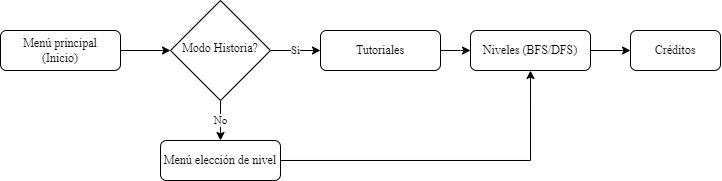
\includegraphics[scale=.5]{imagenes/FlujoDeJuego.png}
	\caption{ Flujo de juego de IGACSE}
	\label{FlujoDeJuego}
\end{figure}


\subsection{Narrativa}

La historia se sitúa en el espacio exterior. Se muestra una nave en un inicio sosteniendo un diálogo con una estación llamada DCC.
La nave está rescatando pandas rojos que están esparcidos en los planetas de la galaxia. El piloto indica que los niveles de combustible están bajos, a lo cual la estación le indica que debería seguir con las siguientes galaxias, pero sin utilizar el pilóto automático, pues las redes neuronales que utilizadas son costosas y consumen combustible. A fin de ahorrar recursos, la nave deberá seguir instrucciones manuales para completar su misión.

Con cada galaxia visitada, el piloto rescata y encuentra otros pandas rojos. Se premia al jugador para que siga con los siguientes niveles y que termine el juego. Los pandas rojos son la mascota del Centro de Alumnos del Departamento de Ciencias  de la Computación (CADCC). Cuando se realizan actividades de bienvenida a los nuevos estudiantes, se muestran afiches con esta mascota \cite{CADCCPage}, por lo que se busca que el jugador se sienta identificado con el juego. Además, la estación se llama DCC para aumentar el sentido de identificación con el jugador, pues DCC son las siglas del Departamento de Ciencias de la Computación \cite{DCCPage}.


\subsection{Menú principal}

El menú principal permite seleccionar idioma apretando el botón en la esquina superior izquierda de la figura \ref{MenuPrincipal}. Los idiomas disponibles son entre inglés y español. Además, proporciona las opciones para jugar el modo historia o los niveles jugables.

\begin{figure}[h]
	\centering
	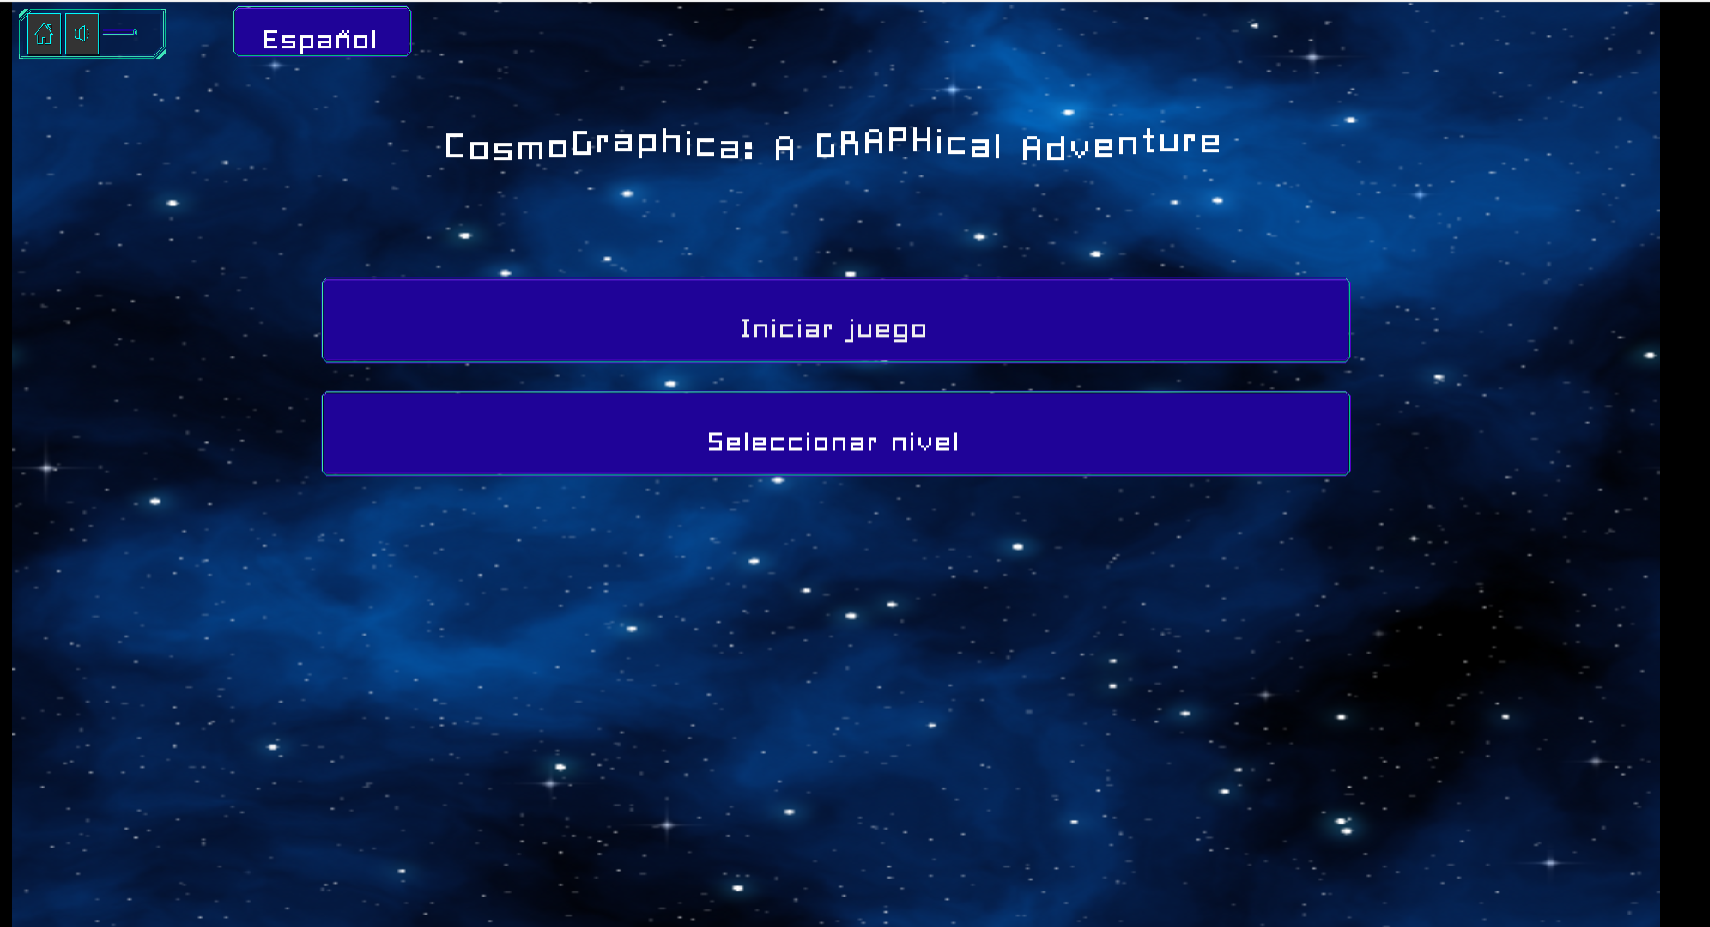
\includegraphics[scale=0.3]{imagenes/MainMenu.png}
	\caption{Menú principal de IGACSE, que se muestra al iniciar el juego.}
	\label{MenuPrincipal}
\end{figure}


\subsection{Tutoriales}

Los tutoriales buscan enseñarle al jugador las mecánicas básicas que serán utilizadas durante le resto del juego. Además, introducen al jugador a la historia, situada en una nave que está rescatando Pandas Rojos esparcidos en los planetas de la galaxia. La historia de fondo busca mostrar una aplicación de los grafos sin explicitar qué contenido se está enseñando.
Las mecánicas se enseñan a través de una combinación de elementos, entre texto y hints visuales, como un mouse haciendo click izquierdo o una tecla R siendo presionada sobre el planeta.
Cada nivel y tutorial es repetible para que el jugador pueda volver a probarlo en caso de no haber entendido algo.

\subsubsection{Primer Tutorial}

El primer tutorial busca enseñar la pantalla y que los planetas son navegables. Que hay caminos que conectan los planetas y se puede hacer click entre ellos. En esta instancia también se enseña sobre el diálogo y se muestran las pistas visuales


\begin{figure}[h]
	\centering
	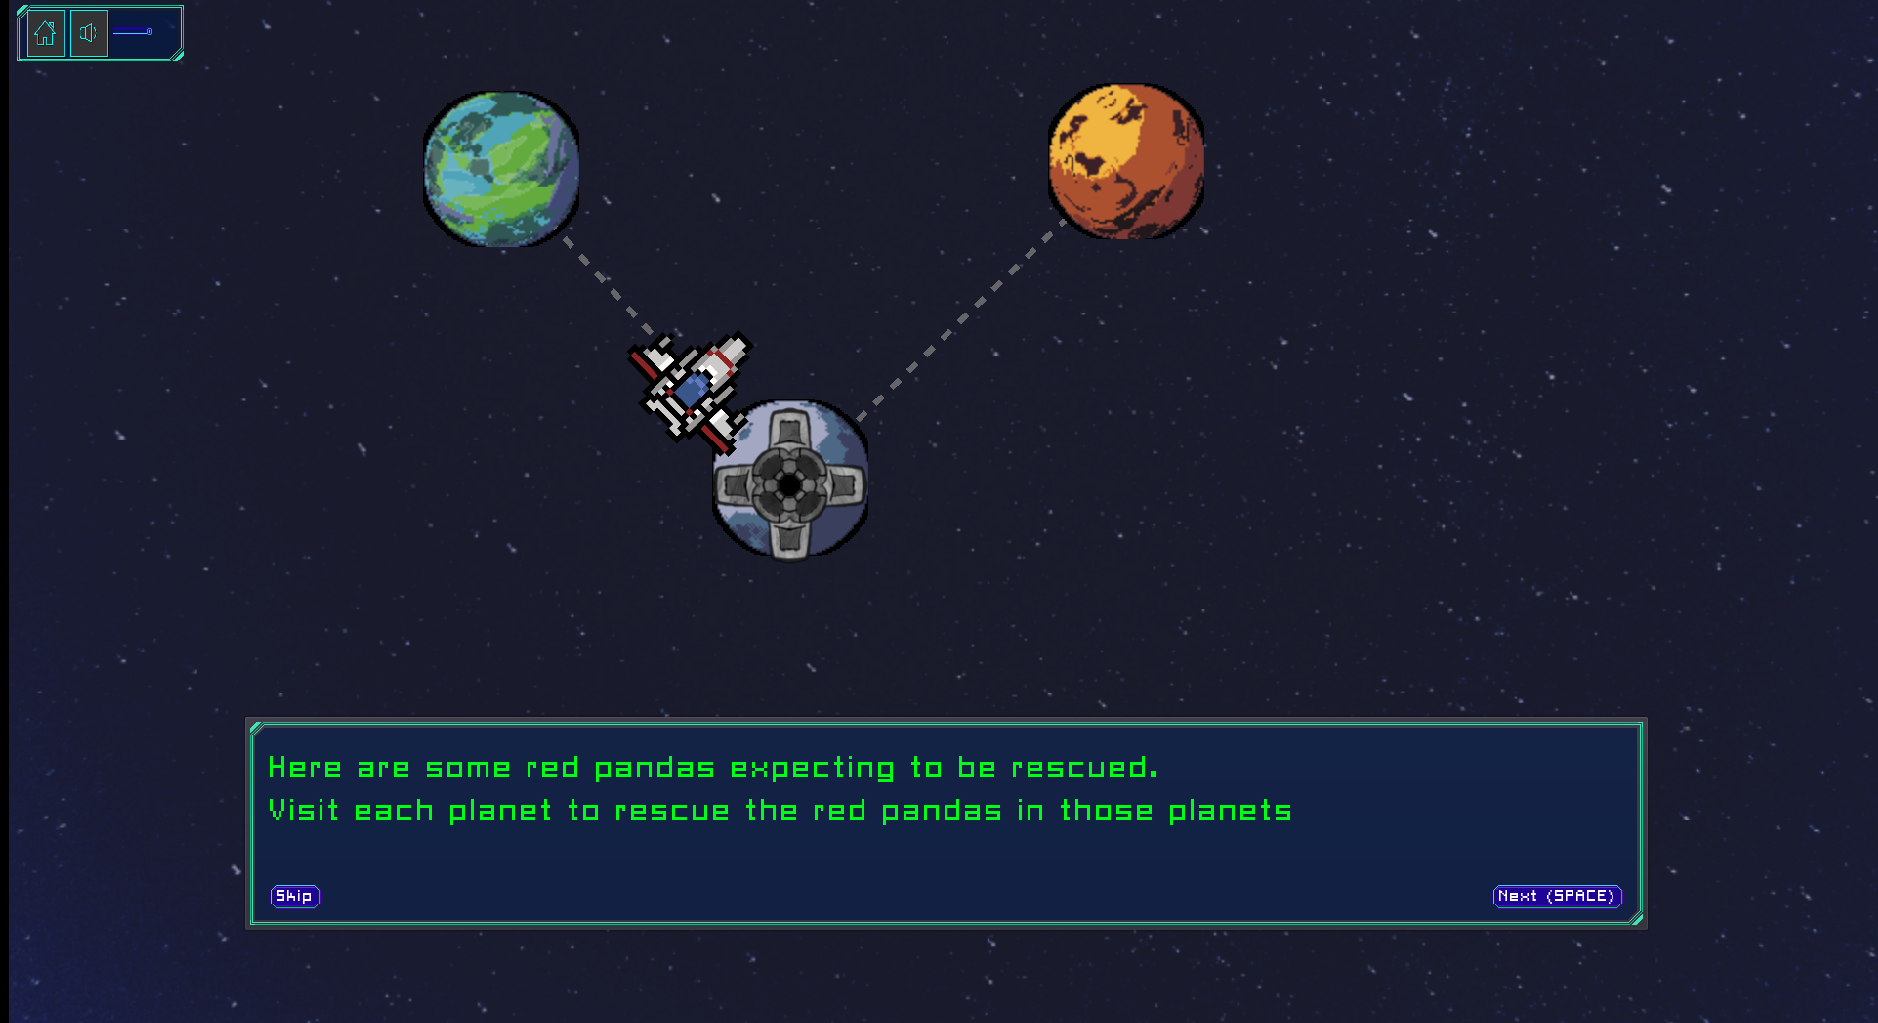
\includegraphics[scale=0.3]{imagenes/FirstTutorial.png}
	\caption{Primer tutorial. Se le indica al jugador a través de un diálogo que debe visitar cada planeta.}
	\label{FirstTutorial}
\end{figure}



\subsubsection{Segundo tutorial}

El segundo tutorial introduce a la mecánica de instrucciones. Además, se introduce al ciclo for y al if en las instrucciones, que serán utilizadas posteriormente.

Al inicio del segundo tutorial, se le indica al jugador que tendrá que seguir las instrucciones del algoritmo, porque la 
exploración automatizada de pandas rojos es costosa y el combustible se está acabando. Las primeras dos instrucciones 
le piden al jugador apretar la tecla espacio para entender que al apretar espacio, se avanza a la siguiente instrucción (Ver figura \ref{SecondTutorial}).

\begin{figure}[h]
	\centering
	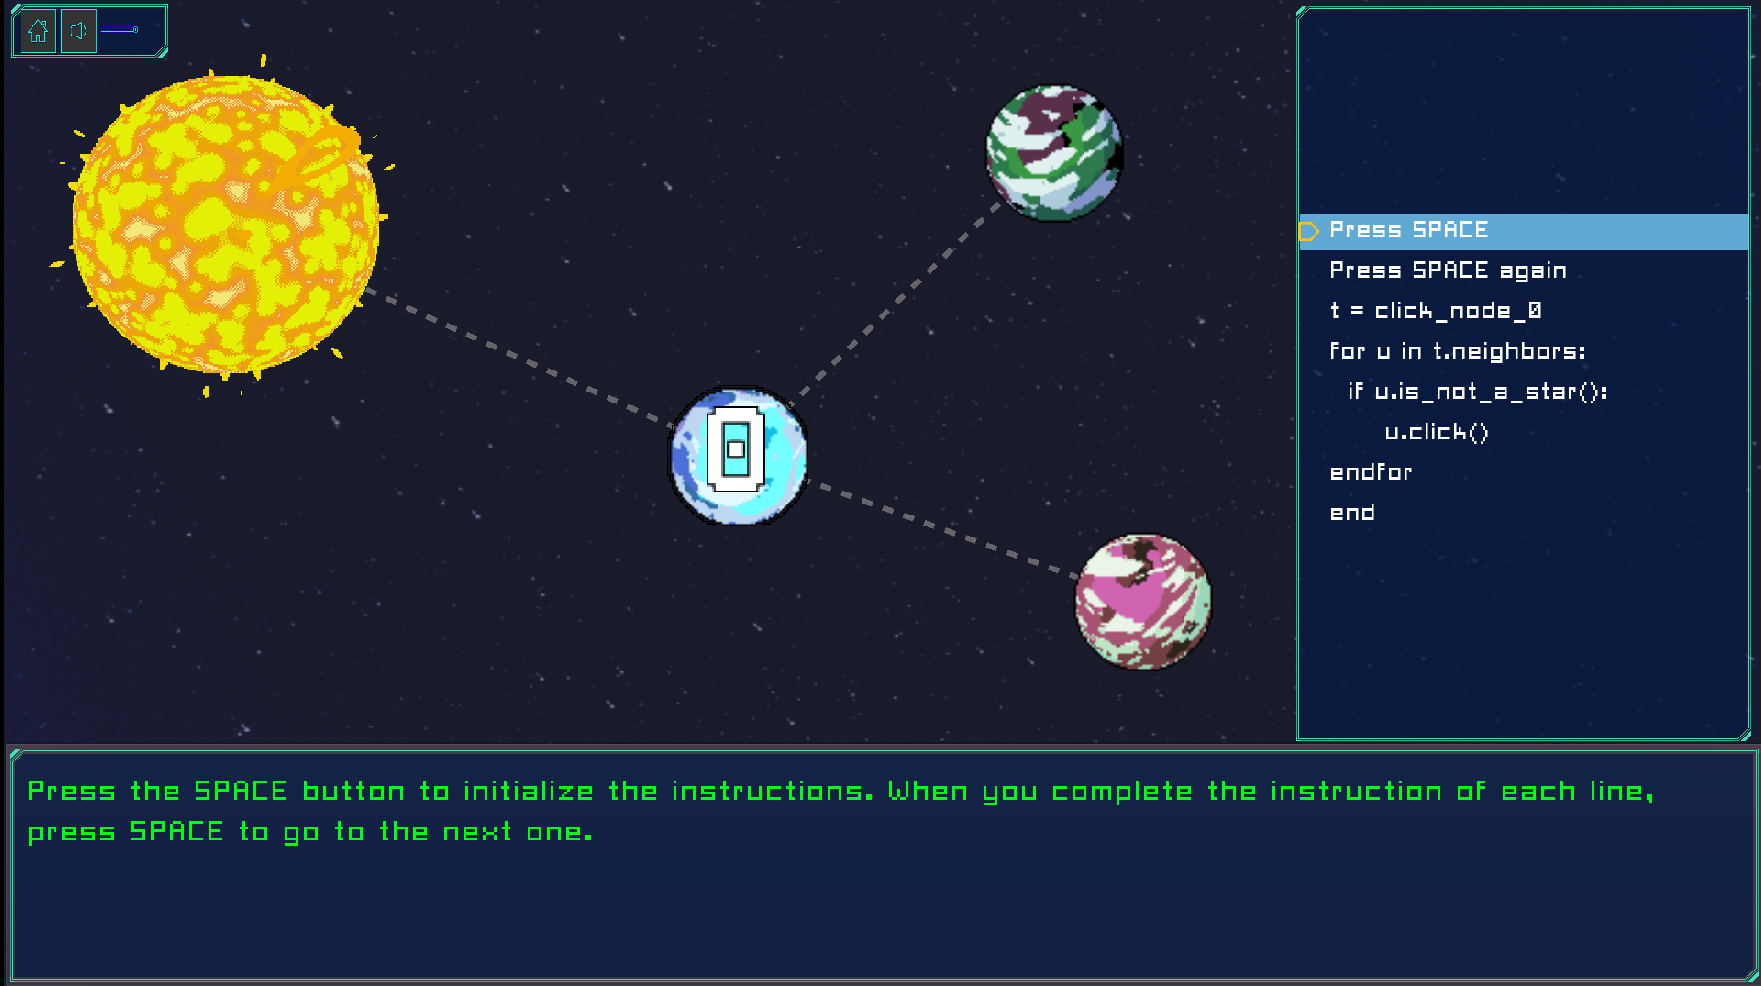
\includegraphics[scale=0.2]{imagenes/SecondTutorial.png}
	\caption{Segundo tutorial. Se le muestra un diálogo de entrada al jugador introduciéndole el nuevo concepto. Este es el primer momento en que se le muestran las instrucciones al jugador.}
	\label{SecondTutorial}
\end{figure}

Durante este segundo tutorial se introduce la lógica de responder sí o no cuando aparece una instrucción con un if en su instrucción. El jugador debe responder correctamente para avanzar a la siguiente instrucción. Si responde incorrectamente, perderá y deberá reiniciar el nivel. En la figura \ref{SecondTutorialShowingIf} se muestra la ventana que le aparece al jugador al llegar a una instrucción con un if.

\begin{figure}[h]
	\centering
	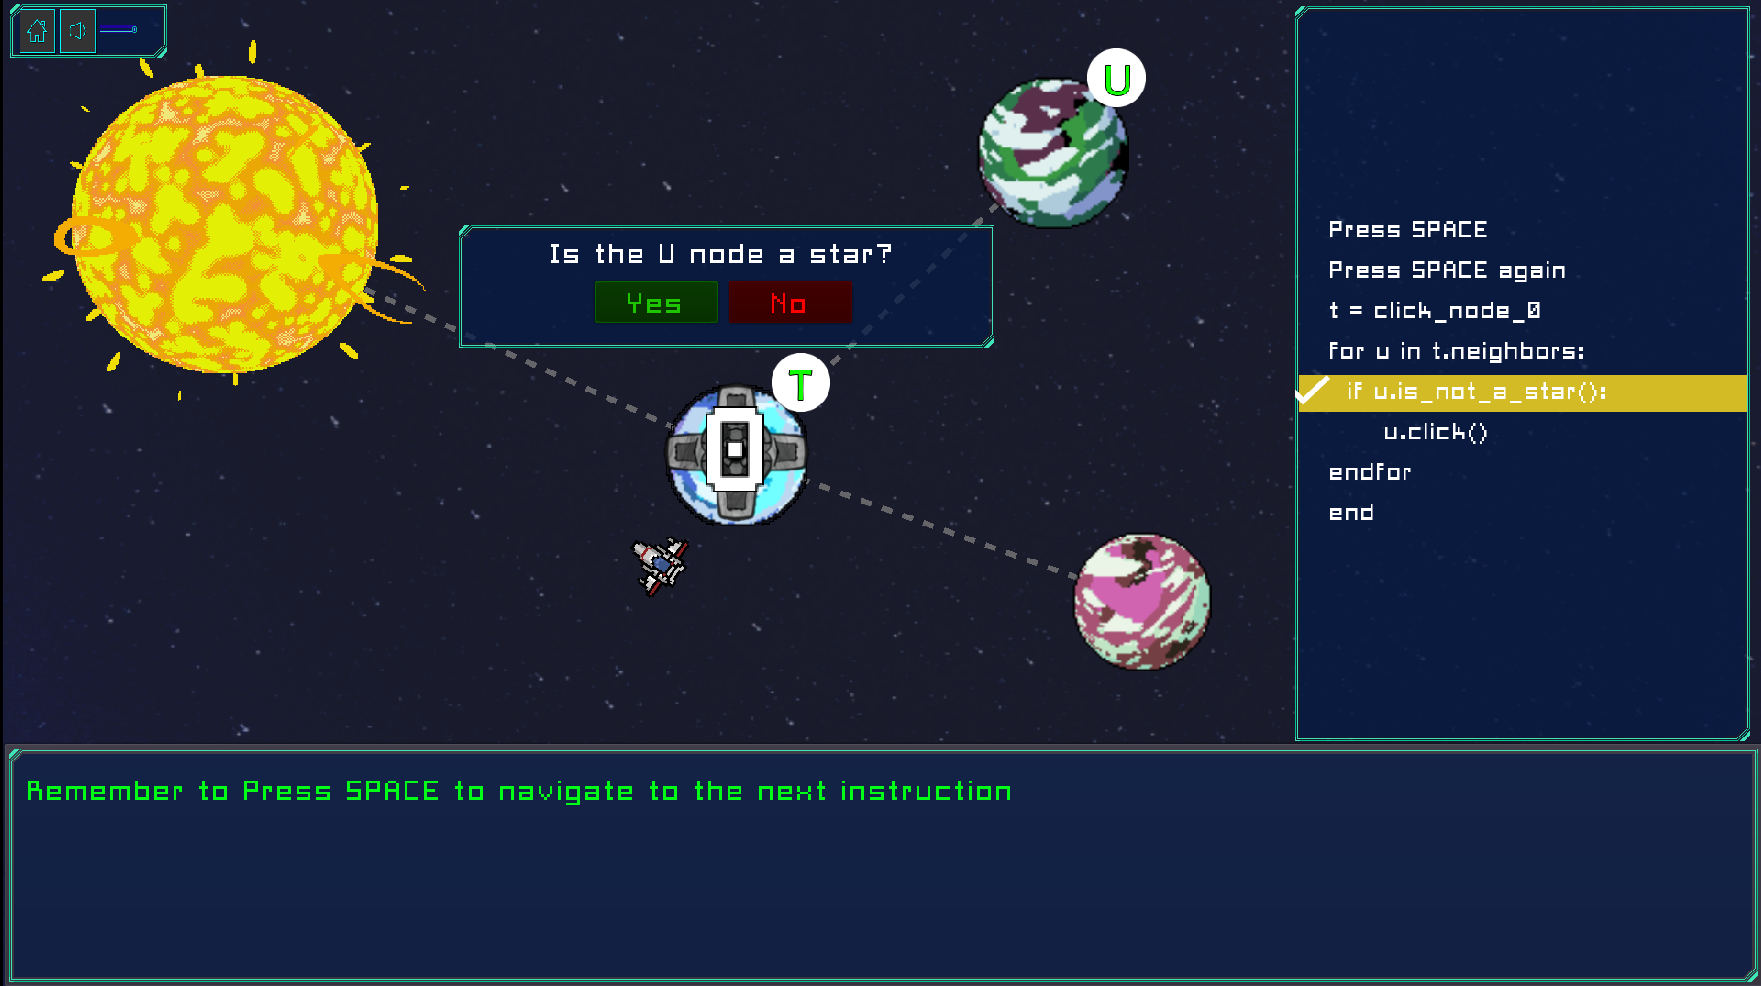
\includegraphics[scale=0.3]{imagenes/SecondTutorialShowingIf.png}
	\caption{Segundo tutorial. Ventana de if que le aparece al jugador al llegar a una instruccion con un if. El jugador debe responder sí o no correctamente para avanzar}
	\label{SecondTutorialShowingIf}
\end{figure}

\subsubsection{Tercer tutorial}

El tercer tutorial introduce al jugador el concepto de Pilas (Stacks) y Colas (Queues) como estructuras de datos para almacenar nodos y luego obtenerlos en órdenes distintos. Además, se le introduce al jugador sobre las variables creadas y la variable seleccionada, la cuak se se usa para señalar a qué objeto se le agregará el nodo que el usuario presione.

\begin{figure}[h]
	\centering
	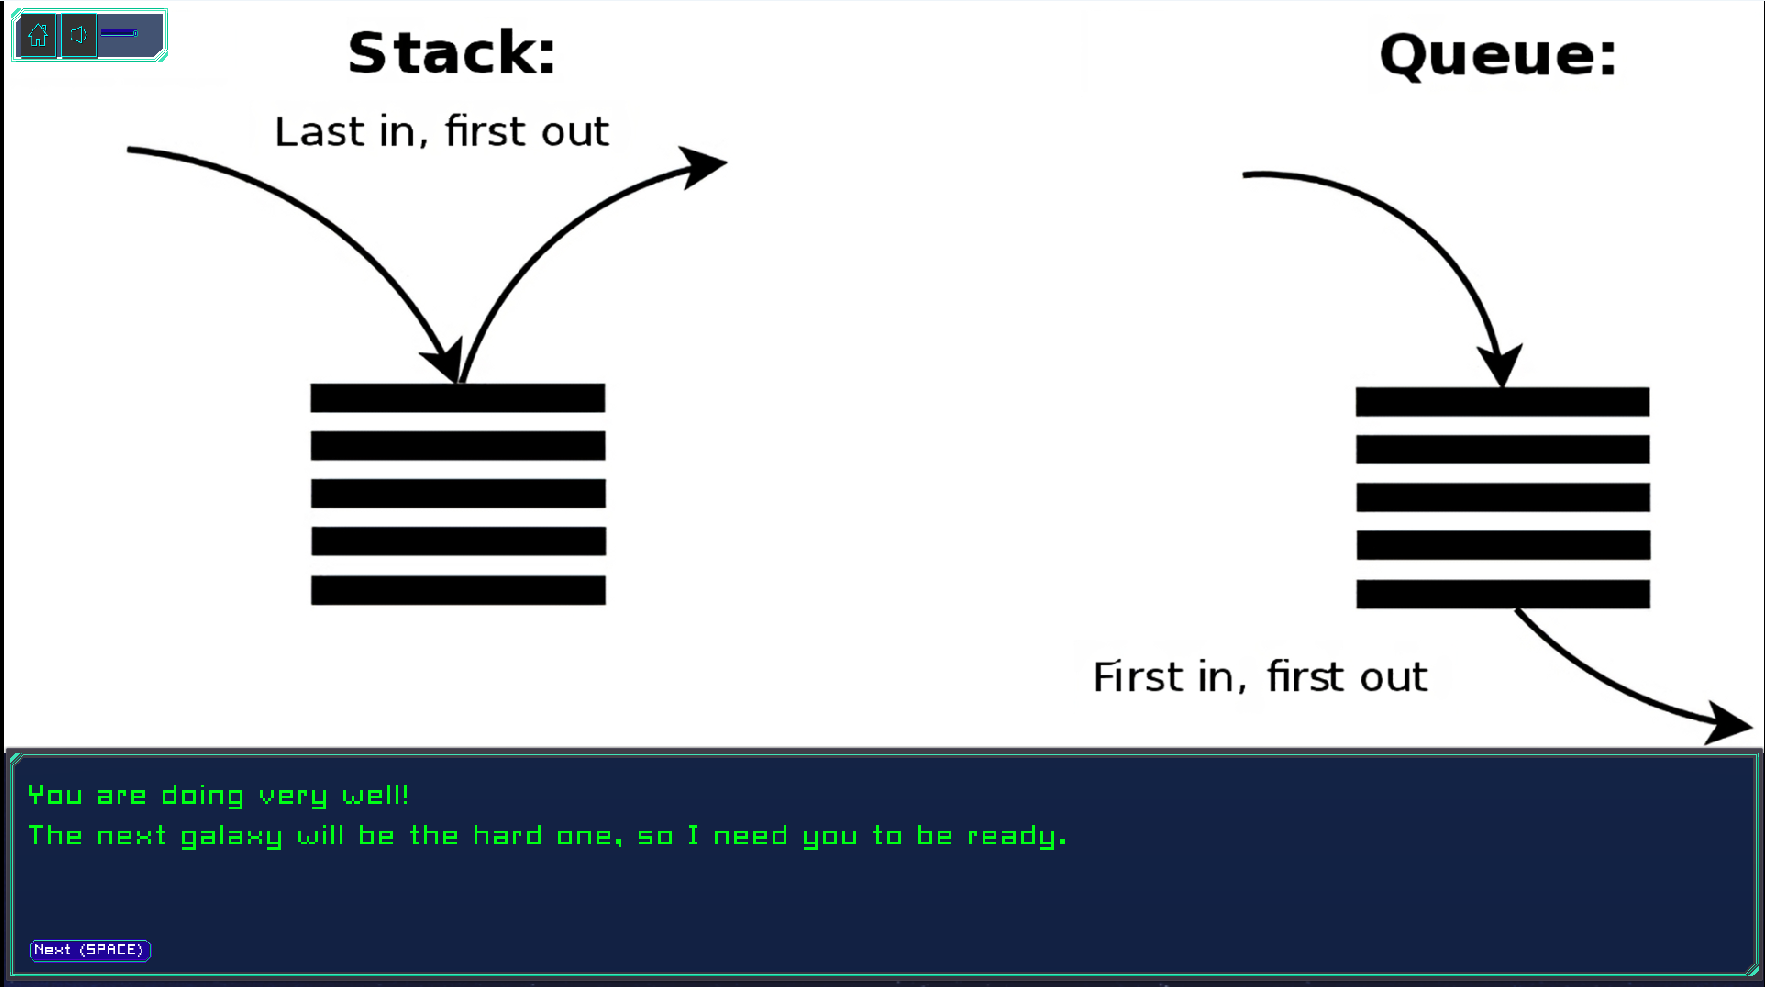
\includegraphics[scale=0.3]{imagenes/ThirdTutorialFirstDialogue.png}
	\caption{Tercer tutorial. Se le explica al usuario al inicio qué son las colas y stacks y cómo funcionan y en qué difieren.}
	\label{ThirdTutorialFirstDialogue}
\end{figure}


\begin{figure}[h]
	\centering
	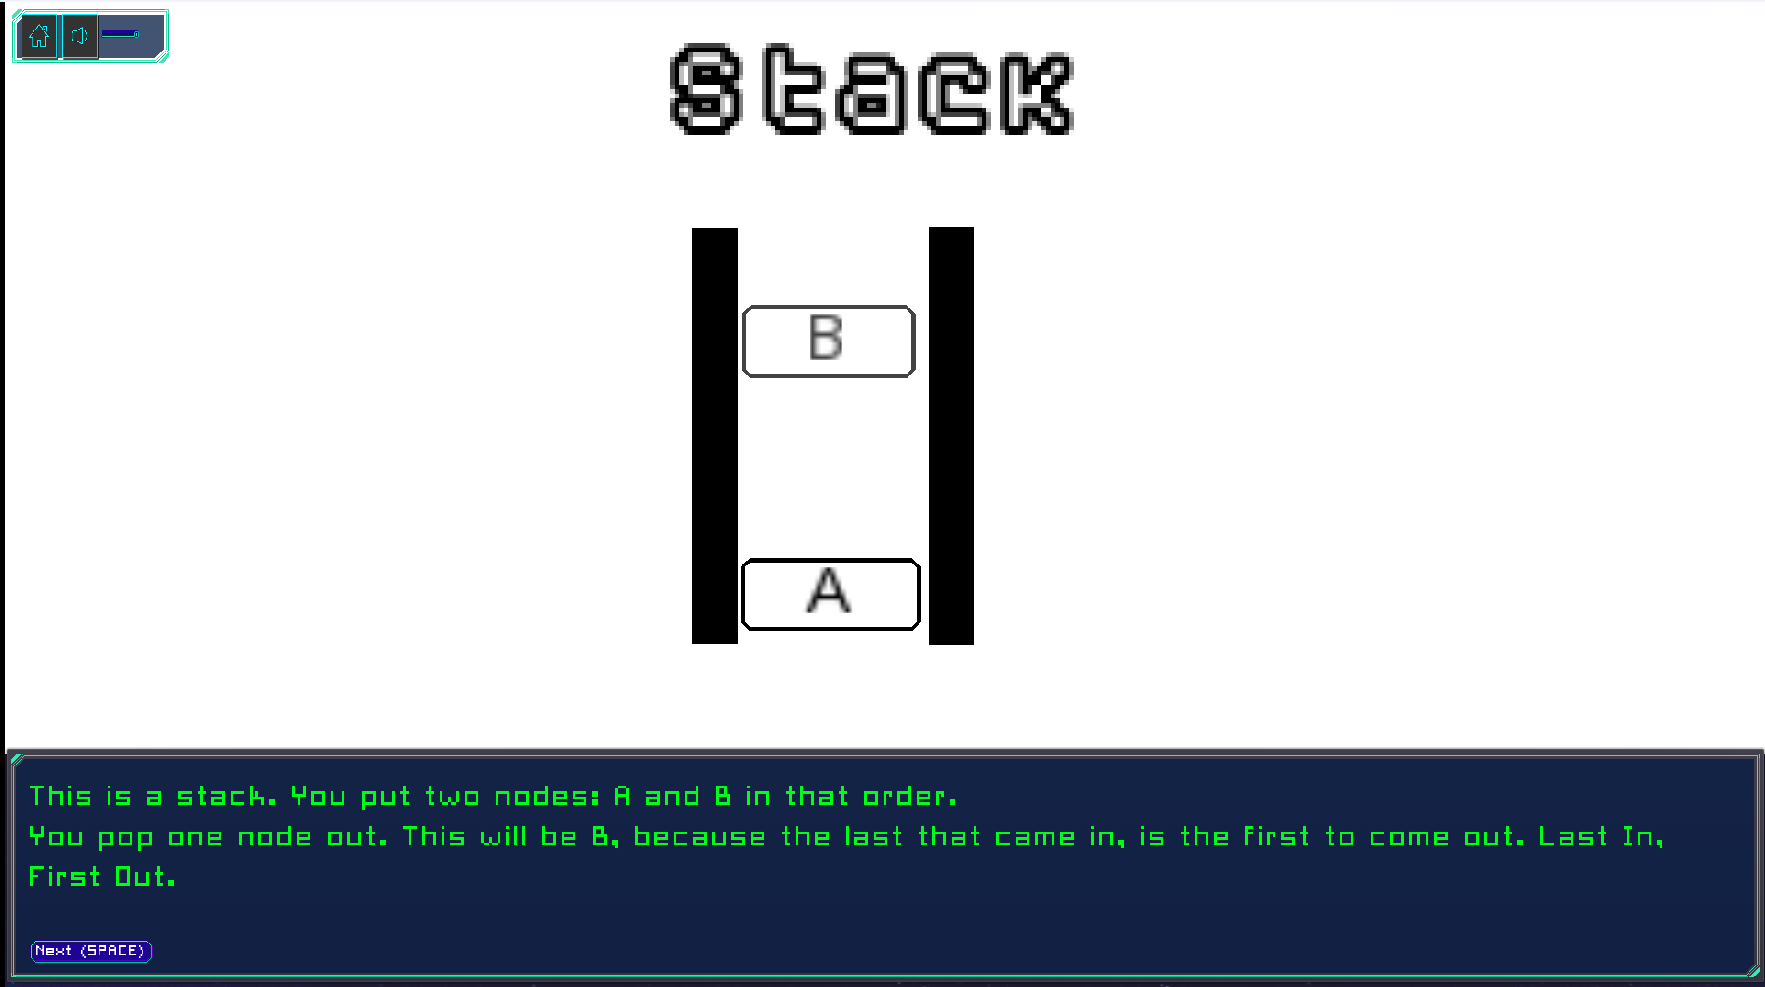
\includegraphics[scale=0.3]{imagenes/ThirdTutorialStackExplanation.png}
	\caption{Tercer tutorial. Mostrando al usuario cómo funciona un stack a través de animaciones.}
	\label{ThirdTutorialStackExplanation}
\end{figure}


El objetivo de las instrucciones en este tutorial es que el jugador aprenda la mecánica para agregar nodos a un stack o a una pila.
Además, se refuerza la mecánica de las instrucciones y ejecutar cada acción paso por paso.


\begin{figure}[h]
	\centering
	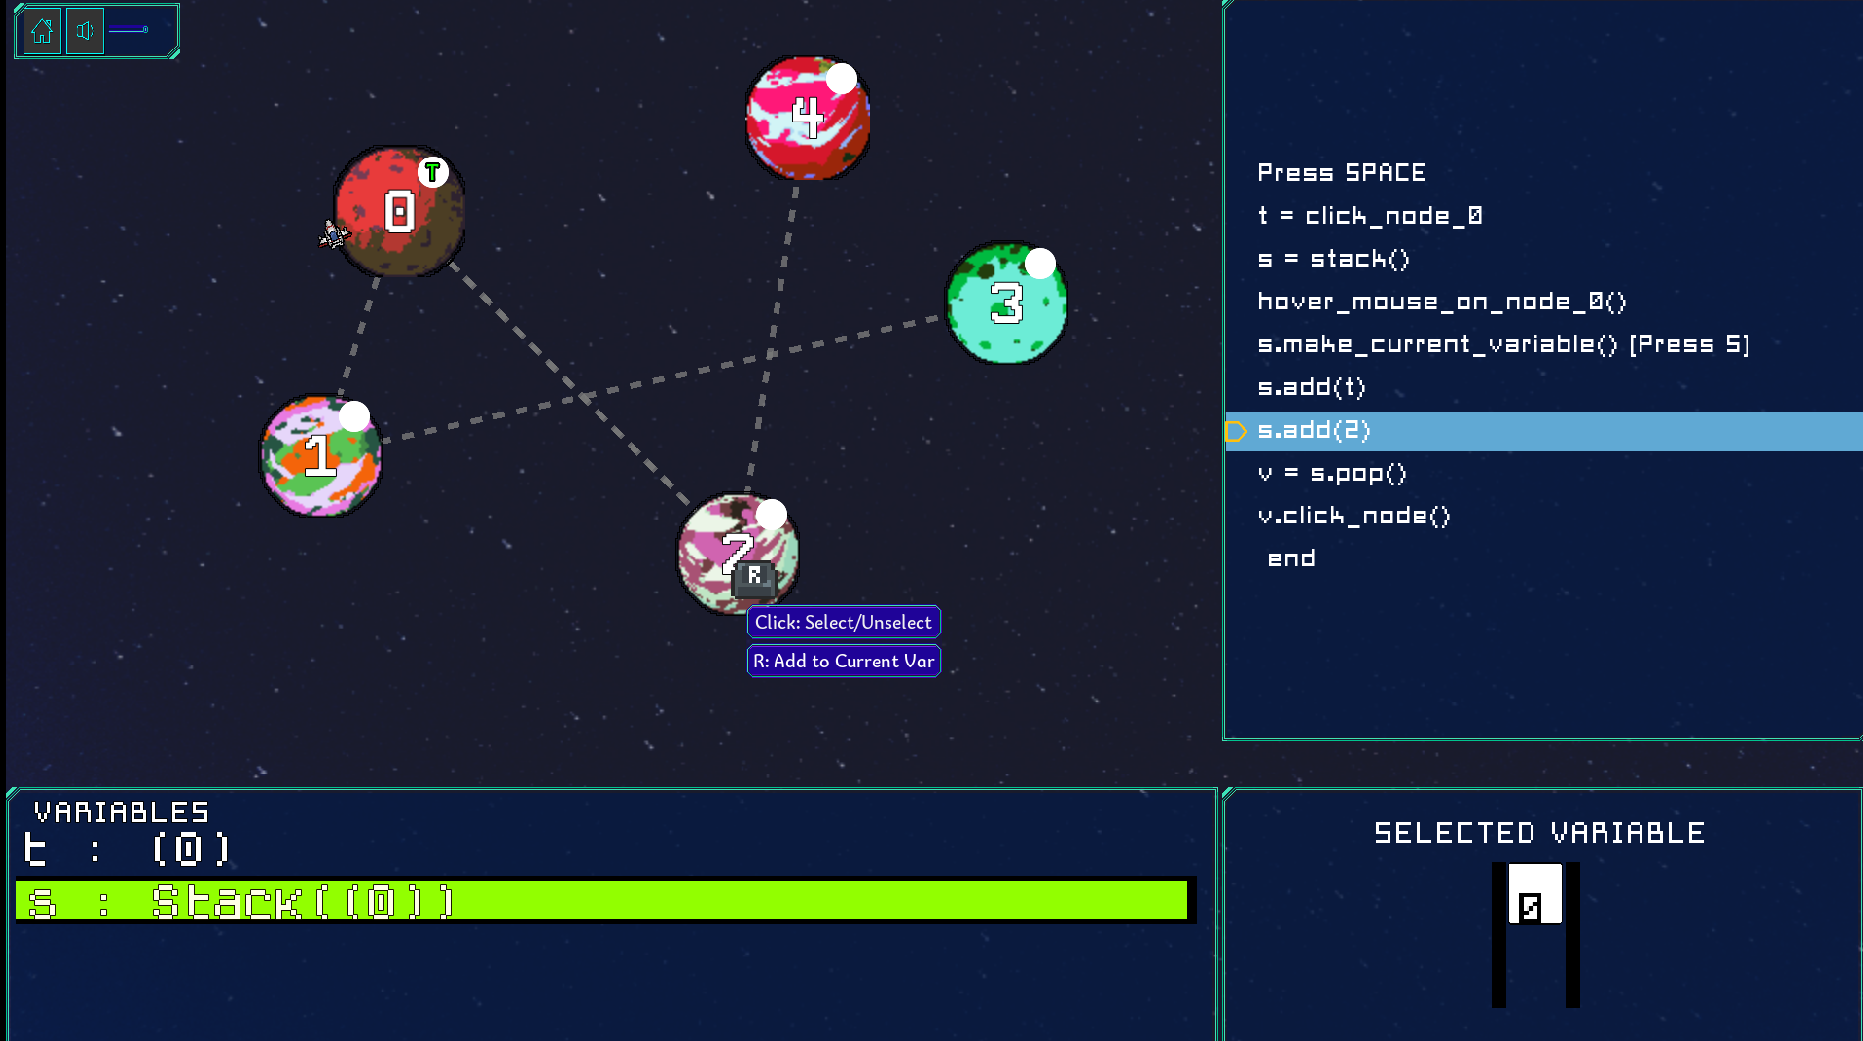
\includegraphics[scale=0.3]{imagenes/ThirdTutorialAddingNode.png}
	\caption{Tercer tutorial. El jugador debe presionar R sobre el planeta 2 para avanzar a la siguiente instrucción.}
	\label{ThirdTutorialAddingNodesToStacks}
\end{figure}


\subsection{Niveles jugables}

Los niveles jugables presentados son BFS y DFS, que enseñan esos algoritmos. Los planetas y sus conexiones son aleatorias, con la restricción de que el grafo formado es siempre es conexo, es decir, todos sus nodos tienen al menos un camino hacia el resto de los otros nodos.

Se crearon 4 niveles para el juego, incluyendo los algoritmos de Kruskal y Prim. Sin embargo, estos últimos no fueron incluidos en la versión final del juego, pues el diseño y la experiencia de usuario eran distintos por requerir otro tipo de acciones, como ordenar arcos y operar con conjuntos, obteniendo uniones e intersecciones. Además, el tiempo de la prueba de usuario era aproximadamente de 45 minutos, por lo que se prefirió no incluirlo en la prueba dado que no se contaba con el tiempo suficiente para probarlos.


\section{Proceso de diseño}

Para diseñar el videojuego, primero se determinaron problemas que se querían solucionar. En particular, el autor del trabajo hipotetiza que los estudiantes de computación no entienden a cabalidad los algoritmos que se enseñan en los cursos de programación, y que no se dan cuenta de que no los entienden. Por lo mismo, se busca que el videojuego sea una herramienta que permita a los estudiantes entender los algoritmos paso a paso, de manera que no se den cuenta de que no los entienden.

En la Universidad de Chile, históricamente y al momento de realizar este trabajo, para entrar a computación se requiere aprobar anteriormente dos años de cursos de plan común, donde existe una práctica conocida como ``pauteo'', la cual consiste en estudiar y revisar pautas de pruebas de semestres pasados para preparase para los exámenes. Con esta práctica, el alumnado revisa las ecuaciones o procedimientos para responder una pregunta sin haber realizado los ejercicios o repetido el procedimiento paso por paso. Muchas veces revisan un algoritmo superficialmente, o lo reproducen mentalmente sin hacerlo en papel. Por lo mismo, se busca que el videojuego sea una herramienta que permita a los estudiantes entender los algoritmos paso a paso y acompañarlo con una visualización.

La idea principal es forzar al usuario a reproducir el algoritmo paso a paso. Esto se puede observar al utilizar el debugger. El debugger permite ver el estado de las variables en cada paso, y permite avanzar paso a paso en el código. El videojuego busca ser una herramienta que permita al usuario reproducir el algoritmo paso a paso, pero de una manera más lúdica. Por esto, el debugger que se utiliza en Visual Studio Code se utilizó como modelo.

% Agregar imagen de debugger en VSCode con un código de Python.

Posteriormente, se realizaron distintos bocetos. Se le mostraron estos bocetos a un diseñador de videojuegos profesional con títulos ya liberados. Se eligió el que fue entendido a primera vista y que se veía más atractivo, además que se parecía más a Visual Studio Code. Se implementaron versiones del videojuego con Godot, que permitía agregar nuevas funcionalidades rápidamente, además de permitir cambiar el estilo. El autor del trabajo mostraba su trabajo de tesis semana a semana en un curso de 20 estudiantes, donde se recibían comentarios del resto de los alumnos.

Una vez definido cierto nivel de avance con todos los algoritmos definidos, se probó con 4 usuarios expertos que ya conocían el algoritmo. Sin embargo, no fueron capaces de seguirlo o comprenderlo a cabalidad, por lo que no se cumpliría el objetivo con personas neófitas en los grafos. Por esta razón, se decidió conseguir la asesoría directa de un diseñador de videojuegos y un diseñador de UX/UI.

Los diseñadores, en entrevistas separadas coincidieron en la necesidad de introducir tutoriales que mostraran los elementos del juego uno a uno, por lo que se decidió agregar tutoriales. Además, se decidió agregar una historia de fondo que permitiera al jugador sentirse identificado con el juego y comprendiera un uso inmediato de estos algoritmos y estructuras. Además, agregar una componente de premiación y gamificación aumentaría la motivación de los usuarios.

Una vez finalizados los tutoriales, agregados los estilos, música y elementos narrativos, se procedió a publicar el videojuego en la plataforma de itch.io \href{https://alasaltum.itch.io/igasce}{IGASCE}, una plataforma de videojuegos y elementos relacionados a videojuegos de creadores con bajos recursos o deel mundo indie. El estilo se compró en itch.io a través de la tienda de assets \url{https://azagaya.itch.io/sci-fi-theme}. Los sonidos también se descargaron a partir de la misma tienda.

% Agregar fotos de distintas versiones del juego

\subsection{Diseño de la interfaz de usuario}

La interfaz de usuario está basada principalmente en el debugger de Visual Studio Code (Ver figura \ref{VScodeDebugger}). Se observa aquí que la instrucción actuál está destacada por un puntero y en color. Además, las variables locales muestran su valor en un formato "nombre: valor". El usuario puede avanzar paso a paso en el código.

\begin{figure}[h]
	\centering
	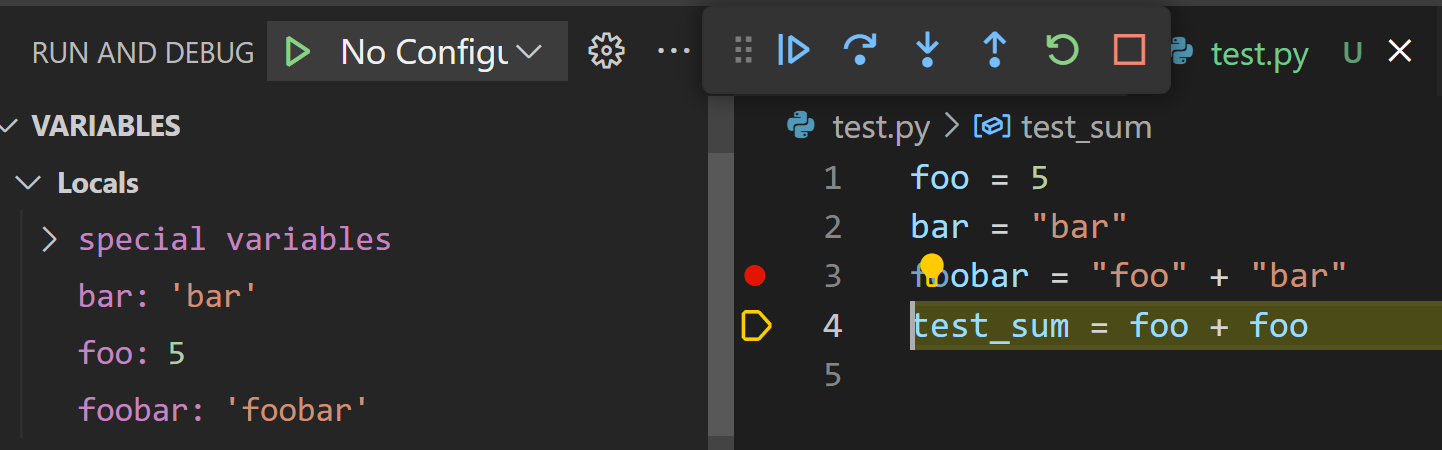
\includegraphics[scale=0.3]{imagenes/VScodeDebugger.png}
	\caption{Visual Studio Code Debugger.}
	\label{VScodeDebugger}
\end{figure}

Hay otros juegos cuya interfaz sirvió de inspiración para la realización del juego final, como 7 Billion Humans, donde el código se ve a la derecha de la pantalla, y la pantalla con los elementos y eventos del juego está al lado izquierdo. Lo que ocurre en la interfaz de la derecha afecta al mundo.

\begin{figure}[h]
	\centering
	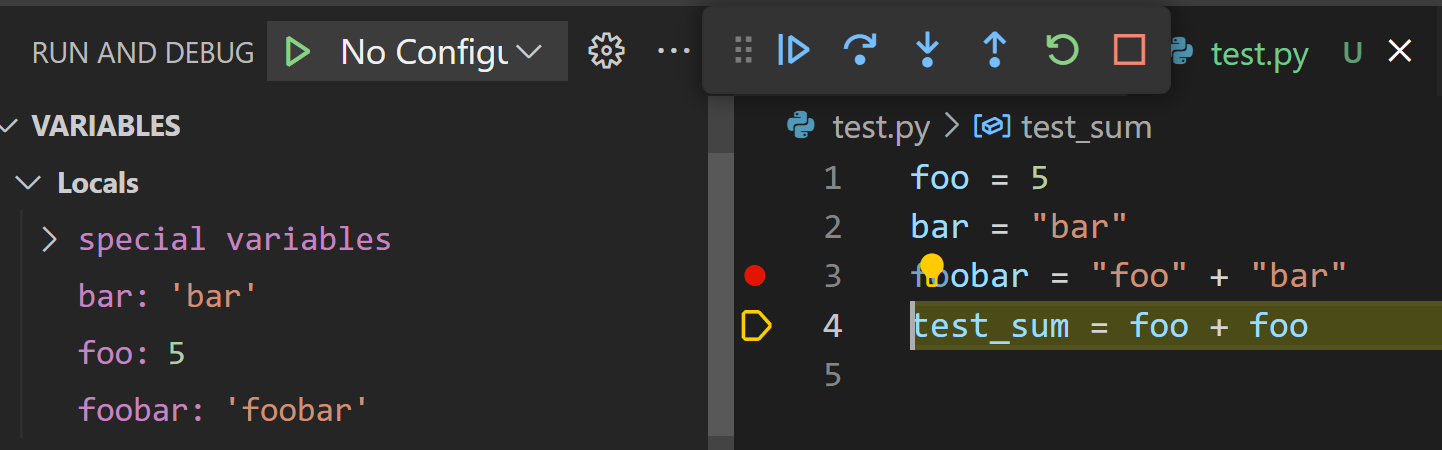
\includegraphics[scale=0.3]{imagenes/VScodeDebugger.png}
	\caption{Videojuego: 7 Billion Humans}
	\label{7BillionHumans}
\end{figure}


Otro videojuego con una interfaz similar es CodeCombat. Aquí el código también está a la derecha, mientras que abajo se ven diálogos y elementos seleccionables. En el caso de IGASCE, los diálogos también se muestran abajo, así como las variables actuales y la seleccionada.
\cite{CodeCombat}. Además, el menú del juego se accede en la esquina superior izquierda (Ver figura \ref{CodeCombat}).

\begin{figure}[h]
	\centering
	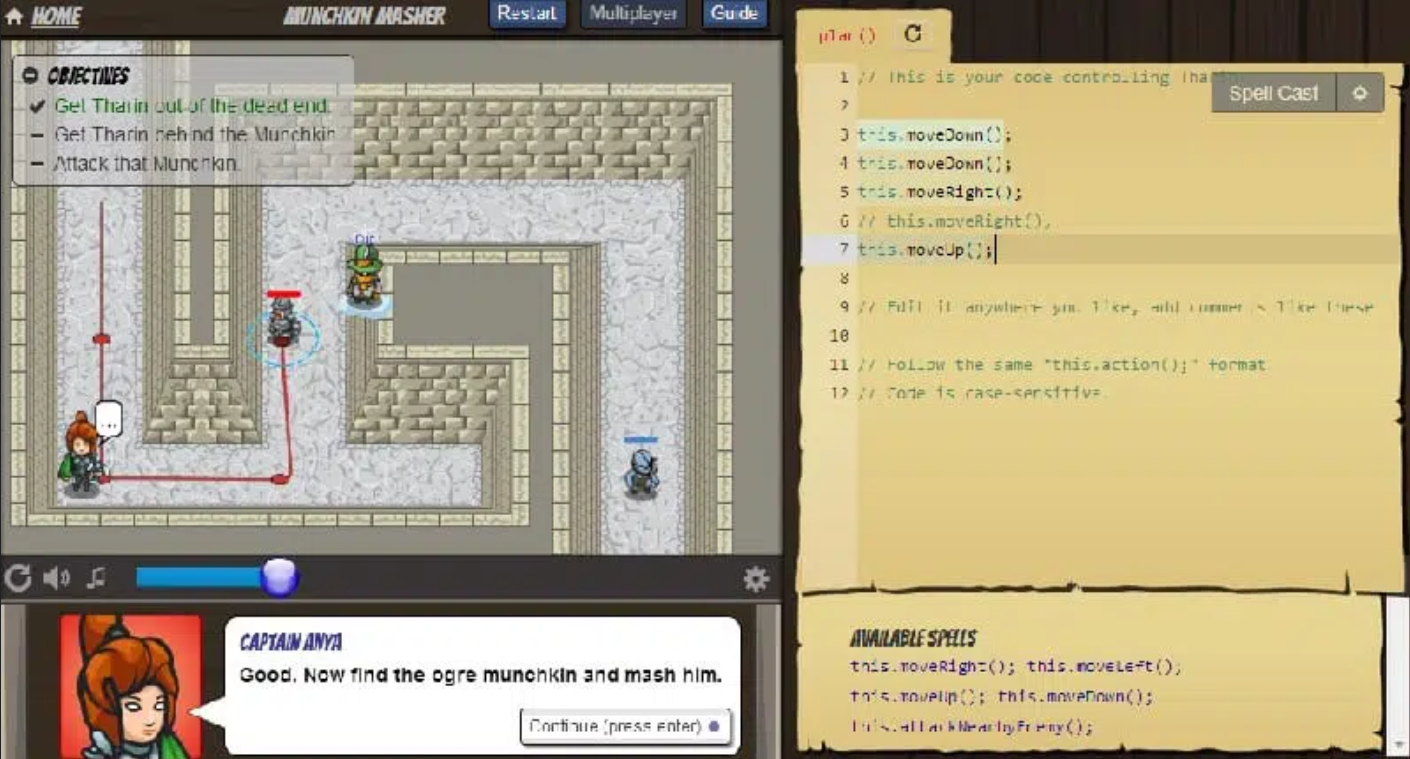
\includegraphics[scale=0.3]{imagenes/CodeCombat.png}
	\caption{Videojuego: CodeCombat}
	\label{CodeCombat}
\end{figure}


\subsection{Diseño de efectos de sonido y música}

Los juegos retro suelen utilizar loops de música de 8 a 16 bits. Algunos ejemplos son: Golden Sun \cite{Wiki_Golden_Sun}, ProtoCorgi \cite{ProtoCorgi}, Pokemon Emerald \cite{PokemonEmerald}, Space Invaders \cite{SpaceInvaders}, o Final Fantasy IV \cite{FinalFantasyIV}.

En el caso de Pokemon \cite{PokemonEmerald}, cada vez que se hace click en algún botón y se gatilla un evento, se emite un sonido de confirmación, como cuando el jugador selecciona un ataque. Lo mismo ocurre en Golden Sun \cite{Wiki_Golden_Sun}. El objetivo es confirmarle al usuario que se está ejecutando correctamente una acción. En el caso de IGASCE, se utilizan sonidos de confirmación cuando se hace click en un planeta o en un camino, o cuando se presiona una tecla correctamente, ya sea espacio o R. Los sonidos de confirmación en todos estos casos son agudos, para que el jugador no se distraiga con ellos, además de dar a entender que la acción tiene un efecto inmediato.

En el caso de los sonidos de error, se utilizan sonidos graves, con fade y que suelen dar la sensación de vibración (Ver figura \ref{EspectroOndasSonidoError}), para que el jugador se dé cuenta que cometió un error y que debe corregirlo. En el caso de IGASCE, se utilizan sonidos de error cuando se hace click en un planeta o en un camino incorrecto, o cuando se presiona una tecla incorrecta, como apretar espacio cuando todavía no se finaliza una instrucción. Además, se utilizan sonidos de error cuando se contesta incorrectamente una pregunta del tipo Sí/No.

\begin{figure}[h]
	\centering
	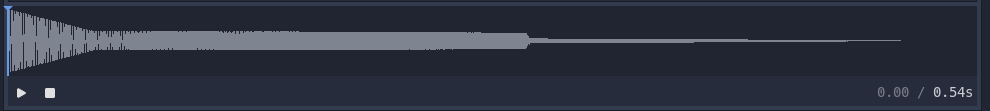
\includegraphics[width=0.9\textwidth]{imagenes/EspectroOndasConfirmacion.png}
	\caption{Espectro de Ondas del sonido de Confirmación de IGASCE}
	\label{EspectroOndasSonidoConfirmacion}
\end{figure}


\begin{figure}[h]
	\centering
	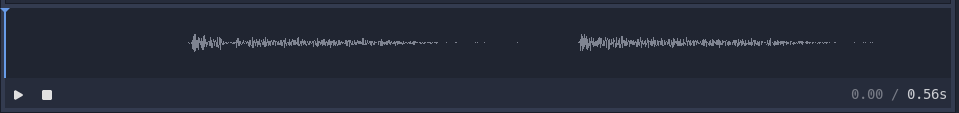
\includegraphics[width=0.9\textwidth]{imagenes/EspectroOndasError.png}
	\caption{Espectro de Ondas del sonido de Error de IGASCE}
	\label{EspectroOndasSonidoError}
\end{figure}


\subsection{Diseño de mecánicas de juego}

% Agregar diagrama de jugabilidad
La mecánica que determina si se gana un nivel o no es cumplir todas las instrucciones presentadas por el algoritmo. Para los niveles BFS y DFS, esto coincide con haber visitado todos los nodos del grafo. El puntero de instrucciones indica la instrucción actual. El jugador debe completar correctamente lo que pide la instrucción, ya sea hacer click, responder una pregunta o agregar un nodo a una estructura de datos, aunque hay instrucciones que no piden ejecutar nada por parte del jugador, como las instrucciones que contienen la palabra clave \textit{for}. Una vez ejecutados correctamente los pasos exigidos, cambiará el color de la instrucción y el cursor de la interfaz se transformará en un ticket.

Para avanzar en las instrucciones, el jugador debe presionar la tecla espacio. Si se apreta la tecla espacio sin haber finalizado la instrucción, se emitirá un sonido de error y el color de la instrucción fluctuará entre rojo y amarillo por un segundo. Si se apreta la tecla espacio cuando se ha finalizado la instrucción, se emitirá un sonido de confirmación y se pasará a la siguiente instrucción. Si se apreta la tecla espacio cuando no hay más instrucciones, se emitirá un sonido de victoria y se permitirá pasar al siguiente nivel o los créditos según corresponda. Este proceso se resume en el diagrama \ref{FlujoMecanicaDeNivel}.

\begin{figure}[h]
	\centering
	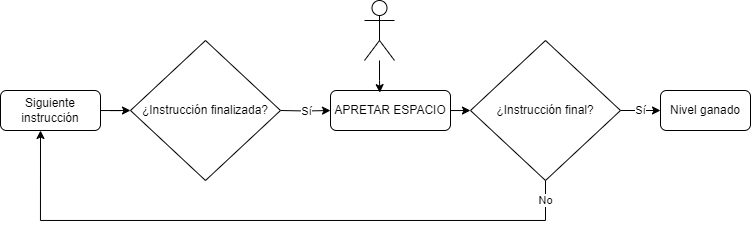
\includegraphics[width=0.9\textwidth]{imagenes/FlujoDeMecanicasDeNivel.drawio.png}
	\caption{Flujo de mecánicas de Nivel. El jugador debe seguir las instrucciones paso a paso.}
	\label{FlujoMecanicaDeNivel}
\end{figure}



\section{Arquitectura de software}

Antes de explicar la arquitectura del programa en específico, es necesario explicar cómo se estructuran los programas hechos en Godot, pues esto justifica las decisiones de diseño tomadas durante el desarrollo de la aplicación.

\subsection{Arquitectura de una aplicación en Godot}

Una aplicación en Godot se construye en base a escenas. Una escena es un conjunto de objetos instanciados al mismo tiempo. Un programa creado en este motor se compone de escenas, que típicamente serán los niveles en un juego. Las escenas tienen un grafo de escena compuesto por uno o más nodos.

Los nodos en Godot son la unidad básica de construcción del programa. Un nodo puede representar un botón, una textura, un reproductor de sonido, áreas de colisión, entre otros. Para armar un personaje que funciona con varios niveles de lógica, tales como: habilidades, movimiento o colisiones, se deben componer más nodos.

La estructura del grafo de escena resulta conveniente en el desarrollo de videojuegos, porque basta mover el nodo padre que representa al personaje, para mover simultáneamente las colisiones, los sonidos y texturas asociadas al personaje. Esto facilita la manipulación de los elementos relacionados.

Otra gran ventaja de usar un motor de videojuegos como Godot es que permite utilizar variables exportadas. Estas son variables cuyo valor se puede definir desde el editor \cite{GodotExportVariables}, lo que permite por ejemplo, instanciar objetos de la misma clase pero con distintas características.


En contraste, cuando se trabaja a un nivel más bajo utilizando bibliotecas como PyGame, que utiliza OpenGL, es necesario abordar cada nivel de representación de un objeto por separado. Por ejemplo, si se desea mover a un personaje con estas bibliotecas, se debe gestionar la textura y las colisiones de manera individual y separada en el código, lo que resulta en un aumento de los costos y la complejidad del desarrollo. En \cite{GodotCollisionsAndRendering} se observa que para armar un personaje básico, se le agrega una componente de colisiones y una visual (Sprite2D) por separado.



\subsection{Arquitectura de software de la aplicación IGASCE}

La aplicación se desarrolla en diferentes fases, donde se pueden identificar 3 tipos de escenas: menús, tutoriales y niveles jugables. En cada fase, se utilizan módulos distintos, y cada nivel, menú o tutorial representa una escena.

Los menúes se basan principalmente en nodos de control, que se utilizan típicamente para interfaces gráficas. En este caso, los menúes consisten únicamente en botones que ejecutan códigos según su descripción, sujetos a ordenadores verticales o en forma de grilla (Ver figura \ref{GodotMenuInterface}).

\begin{figure}[h]
	\centering
	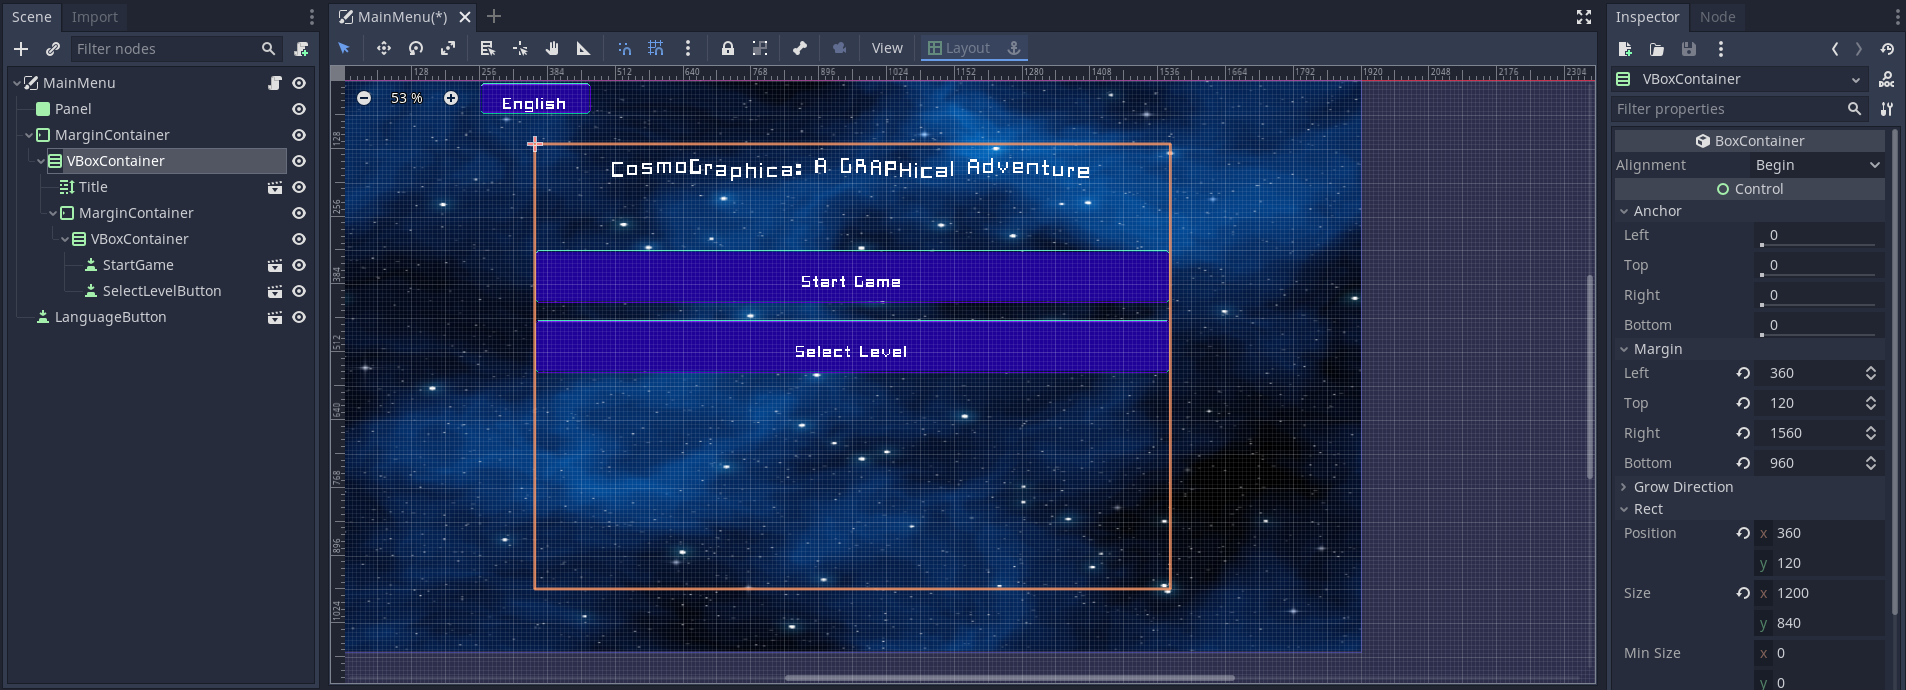
\includegraphics[width=0.9\textwidth]{imagenes/GodotInterfaceMainMenu.png}
	\caption{Interfaz de Godot describiendo la escena del menú principal de IGASCE. El juego públicamente se dio a conocer como CosmoGraphica, pero el proyecto completo se llama IGASCE.}
	\label{GodotMenuInterface}
\end{figure}


Los tutoriales tienen una lógica más compleja y son similares a los niveles. La diferencia con las escenas finales es que los tutoriales incluyen una ventana de diálogo que busca conectar la historia del videojuego con los elementos interactivos, además de que el grafo ya está predeterminado, por lo que los nodos y arcos ya vienen predefinidos.

\begin{figure}[h]
	\centering
	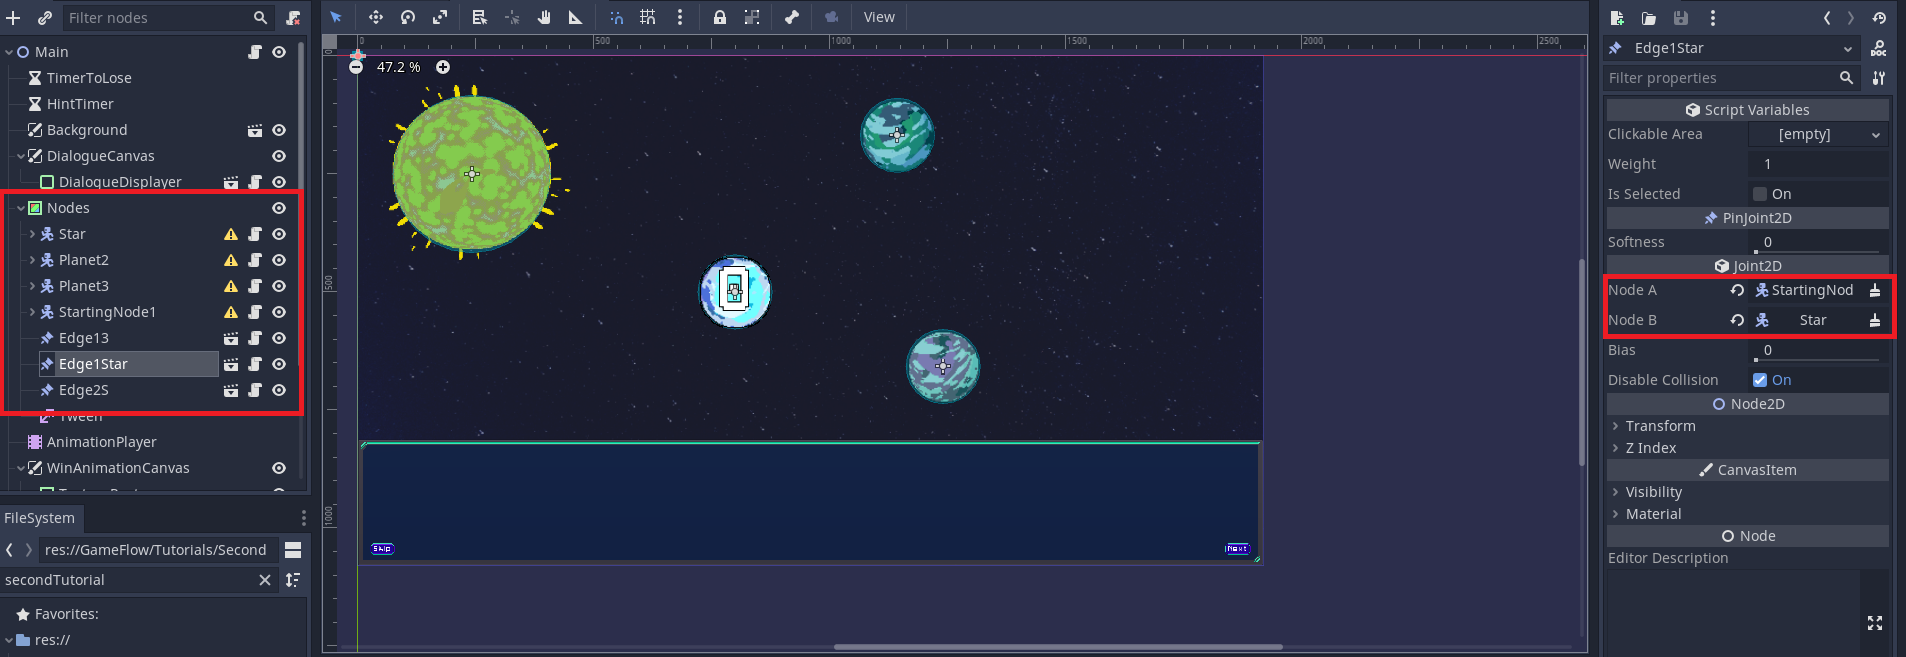
\includegraphics[width=0.9\textwidth]{imagenes/SecondTutorialGraph.png}
	\caption{Interfaz de Godot describiendo el segundo tutorial. En rojo se observa el grafo de escena con los nodos y los arcos ya predefinidos a la izquierda. En la derecha se muestra cómo se unen los arcos, indicando los dos extremos del arco a través de variables exportadas de Godot.}
	\label{SecondTutorialGraph}
\end{figure}


Respecto a los niveles jugables, existen diversos elementos destacables. Entre estos, se encuentran: El código, las variables, la variable seleccionada y la ventana de juego.

En relación al código que se muestra a la derecha de la pantalla durante el juego, este está controlado por un nodo de la clase CodeContainer. Este objeto se encarga de recibir el input del jugador para avanzar en el código. Si las acciones ejecutadas son correctas, el usuario pasa a la siguiente instrucción, desbloqueando nuevas tareas a realizar. La clase CodeContainer posee un arreglo de objetos del tipo CodeLine llamado code\_lines. La clase CodeLine contiene toda la lógica de una única línea de código. Entre sus funciones se encuentran: darle énfasis a la línea de código actual, darle feedback al usuario cuando la instrucción de la línea se completó correctamente y verificar constantemente si la instrucción de línea se ha completado correctamente (ver figura \ref{CodeLinesArchitecture}).

\begin{figure}[h]
	\centering
	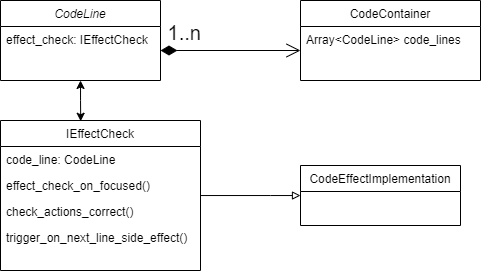
\includegraphics[width=0.9\textwidth]{imagenes/CodeLinesArchitecture.png}
	\caption{Arquitectura de la ejecución de código dentro del juego.}
	\label{CodeLinesArchitecture}
\end{figure}

Cada CodeLine posee un script que se puede indicar desde el editor de Godot a través de una variable exportada. Este script debe heredar de la clase EffectCheck, la cual actúa como interfaz. Cada script que implemente la interfaz EffectCheck debe definir métodos para cuando: 1) El puntero de instrucción llega a la línea del script. 2) Para verificar que la instrucción actual ha sido realizada correctamente. 3) Si corresponde, efectos colaterales de la instrucción. Este último se usa en los ciclos for, donde se mueve el índice utilizado para avanzar por los ciclos y recorrer arreglos. También se utiliza para la creación de variables.

En el panel inferior se encuentran dos clases: DebugBlock y ADTShower. El primero se encarga de mostrar las variables instanciadas, su nombre y su valor actual. Contiene la lógica para agregar, modificar o eliminar alguna variable. Cada vez que se pasa por un ciclo for o se declara una variable, este modifica sus variables internas. Existe una variable seleccionada, la cual puede ser manipulada por el usuario de distintas formas. Al apretar la flecha arriba se selecciona la variable que esté arriba de la actual y viceversa para la flecha de abajo. En la figura \ref{BFSFullGame} se observa que está la variable ``q'' seleccionada.

\begin{figure}[h]
	\centering
	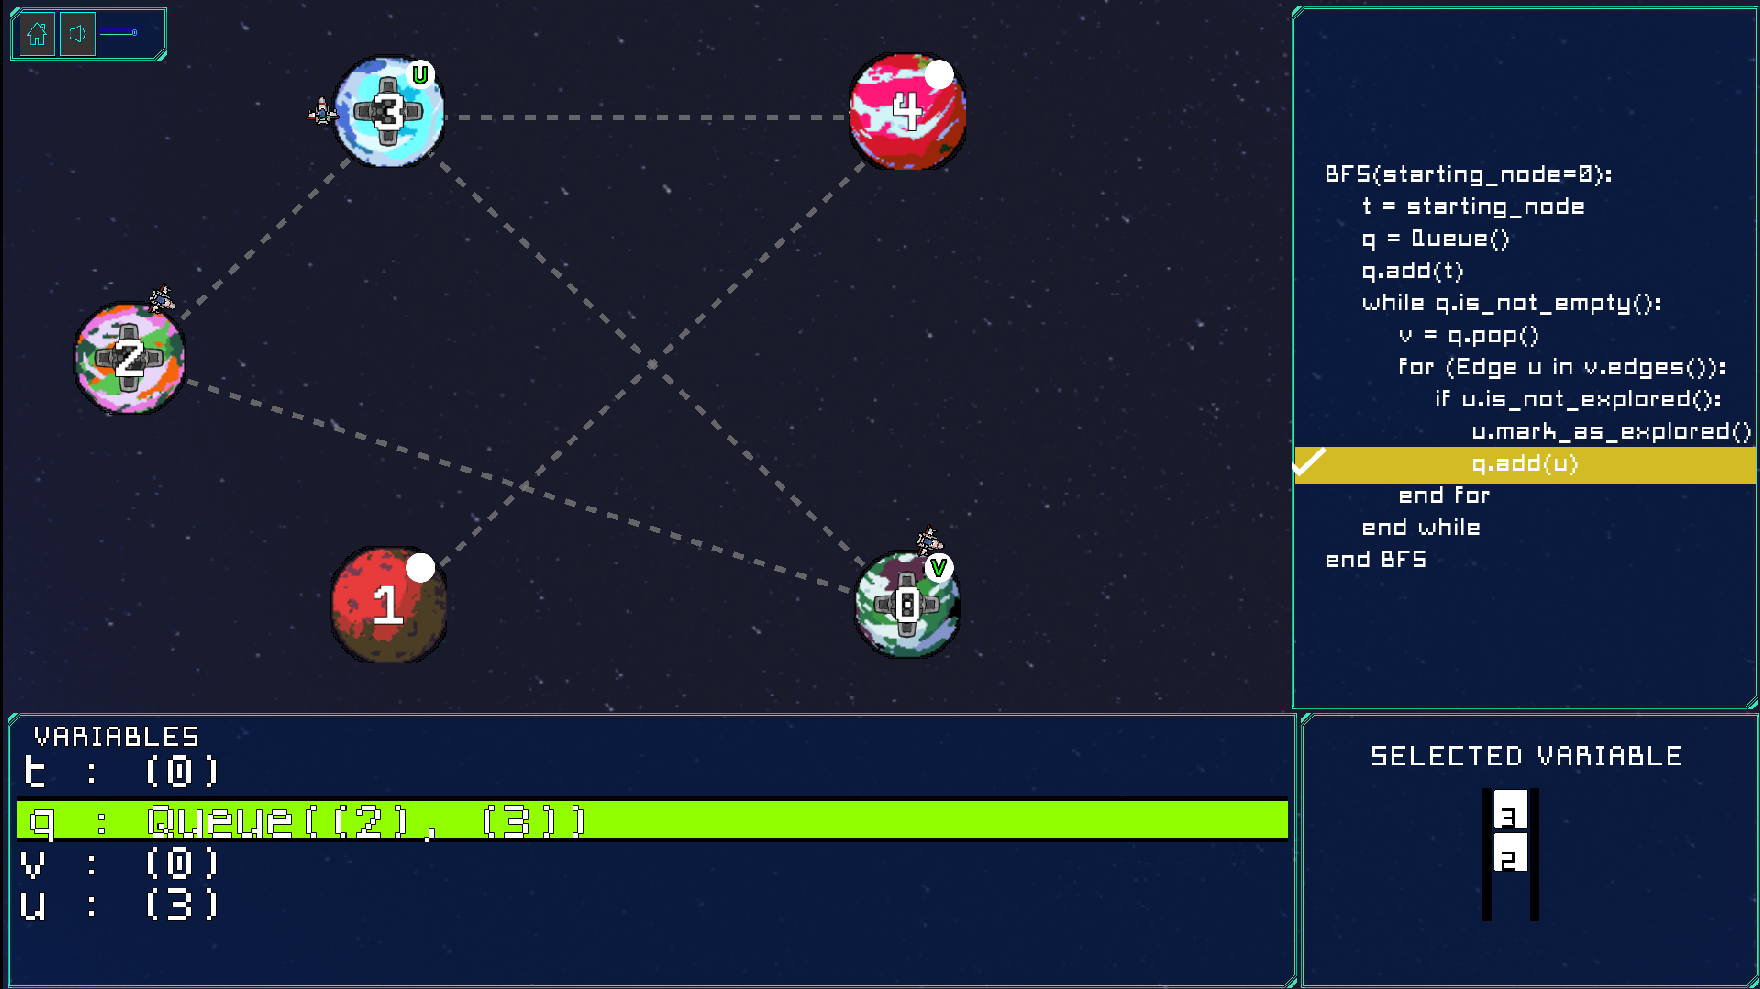
\includegraphics[width=0.9\textwidth]{imagenes/BFSFullGame.png}
	\caption{Nivel jugable BFS. Se observa el código a la derecha, el grafo en el centro, el DebugBlock en la parte inferior izquierda y el ADTShower en la esquina inferior derecha. La varible q está seleccionada.}
	\label{BFSFullGame}
\end{figure}

La clase ADTShower se encarga de mostrar la variable seleccionada por el usuario en el DebugBlock. Este busca agregar una representación visual al objeto seleccionado, para permitir arrastrar nodos a la cola o la pila según el algoritmo que se esté enseñando, BFS o DFS, respectivamente.

Inicialmente, cada cambio en el código por el efecto de alguna CodeLine o línea de código del juego requería modificar las clases DebugBlock, ADTShower, StoredData (Explicada más adelante) y afectar la misma línea de código. Además, estos efectos debían traspasarse a las siguientes líneas de código para lograr cohesión. Por ejemplo, si la línea cinco creaba la variable u y la sexta la modificaba, esto se debía reflejar correctamente en todas las estructuras mencionadas.

Para solucionar el problema del alto costo de implementación, se optó por crear una clase llamada ADTMediator, de acuerdo al Mediator Pattern \cite{Freeman2015TheMP}. Esta clase se inspiró en la arquitectura de React, donde el código generado por React funciona como una Fuente de toda verdad o "Single Source of Truth" \cite{ReactSingleSourceOfTruth}. Con este tipo de arquitectura, se le envía un mensaje a ADTMediator solicitando modificar, crear o eliminar una variable. Esta clase modifica sus variables internas, luego informa a las clases DebugBlock y ADTShower qué mostrar. Una desventaja de esta arquitectura, es que realiza copias innecesarias en cada paso, perdiendo eficiencia. Sin embargo, como se trabaja con pocas variables, este costo no se nota a nivel de usuario. 


\begin{figure}[h]
	\centering
	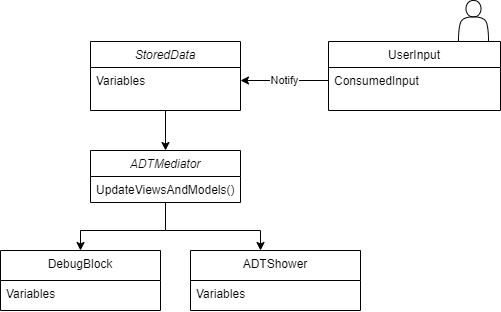
\includegraphics[width=0.9\textwidth]{imagenes/ArquitecturaMediatorAfter.png}
	\caption{Arquitectura de software de un nivel utilizando el ADTMediator, reduciendo el acoplamiento entre clases.}
	\label{ArquitecturaMediatorAfter}
\end{figure}

Una clase que sirve de puente para comunicarse con el ADTMediator es StoredData. Este es un singleton que contiene datos como los avances del usuario en los distintos niveles y el estado del juego. Cuando una línea de código quiere modificar variables dentro del juego, ejecuta un método de este singleton, el cual reenvía esta información al ADTMediator. Esto se hace así porque es fácil obtener el puntero a StoredData, ya que usa el patrón singleton.

Otros singletons son: AudioPlayer, encargado de emitir sonidos específicos en cualquier momento del juego y NotificationManager, que genera ventanas emergentes para el usuario, como menúes, avisos o pestañas donde se debe responder sí o no. Además, se encarga del paso entre niveles.